
\documentclass{article}

\usepackage{amssymb}
\usepackage{amsmath}
\usepackage{pgfplots}
\usepackage{tikz}
\usepackage[top=0.9in, bottom=0.9in, left=1.5in, right=1.5in]{geometry}
\usepackage{xcolor}
\usepackage{xparse,mathtools}



\title{ECE421 Problem Set 2}
\author{Micol Altomare}
\date{September 27, 2023} 

\begin{document}

\maketitle


\section{Linear Regression}

Given data:

\begin{table}[htbp]
   \centering
   %\topcaption{Table captions are better up top} % requires the topcapt package
   \begin{tabular}{|c|c|} % Column formatting, @{} suppresses leading/trailing space
   \hline
      $x^{(i))}$    & $t^{(i)})$  \\ 
      \hline \hline
      1 & 6  \\
      2 & 4     \\
      3 & 2   \\
      4 & 1  \\
      5 & 3 \\
      6 & 6 \\
      7 & 10 \\
      \hline
   \end{tabular}
   \caption{Given data}
   \label{tab:booktabs}
\end{table}

\subsection{}

\begin{figure}[ht]
  \centering
  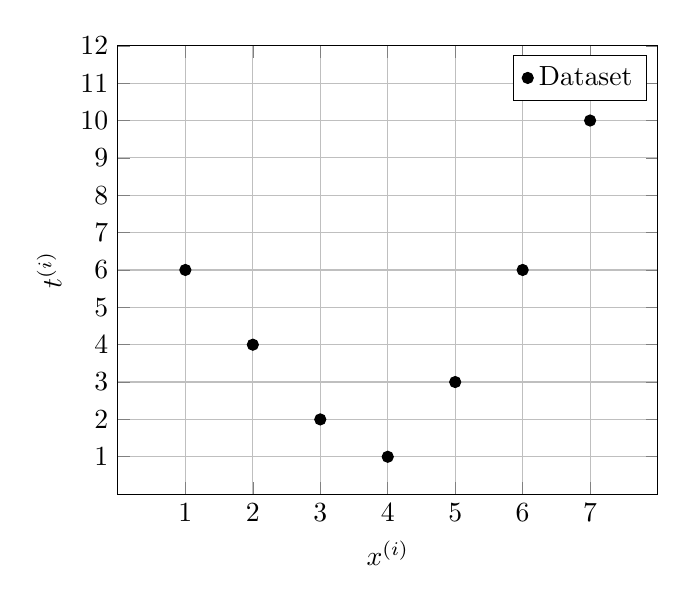
\begin{tikzpicture}
    \begin{axis}[
      xlabel={$x^{(i)}$},
      ylabel={$t^{(i)}$},
      xmin=0, xmax=8, 
      ymin=0, ymax=12,
      xtick={1,2,3,4,5,6,7},
      ytick={1,2,3,4,5,6,7,8,9,10,11,12},
      grid=both,
      mark=*,
      ]
      
      \addplot[only marks] table {
        1 6
        2 4
        3 2
        4 1
        5 3
        6 6
        7 10
      };
      \addlegendentry{Dataset}
	% question 1.5
      %\addplot [dotted, domain=0:8, samples=2, ultra thick] {0.607142857*x + 2.142857143};
      %\addlegendentry{Linear regression} //// mark=*????
    \end{axis}
  \end{tikzpicture}
  \caption{Scatter plot of $x^{(i)}$ vs. $t^{(i)}$}
\end{figure}


\subsection{}

\begin{align*}
\mathcal{E} (w, b) &= \frac{1}{2N} \sum_{i = 1}^{N} (y^{(i)} - t^{(i)})^2 \\
&=  \frac{1}{2N} \sum_{i = 1}^{N} (wx^{(i)} - t^{(i)})^2 \\
&= \frac{1}{2N}  \sum_{i = 1}^{N}  \left[ (wx^{(i)})^2 + wx^{(i)}b -wx^{(i)} t^{(i)} + wx^{(i)}b + b^2 - bt^{(i)} - wx^{(i)}t^{(i)} - t^{(i)}b + (t^{(i)})^2 \right] \\
&= \frac{1}{2N}  \sum_{i = 1}^{N}  \left[ (w^2 x^{(i)})^2 + 2wx^{(i)} b - 2w x^{(i)} t^{(i)} - 2bt^{(i)} + b^2 + (t^{(i)})^2 \right] \\
&= \boxed{ \frac{1}{2N}  \sum_{i = 1}^{N} \left[ \textcolor{blue}{(x^{(i)})^2} w^2 + \textcolor{blue}{1}b^2 + \textcolor{blue}{2x^{(i)}}wb  \textcolor{blue}{-2t^{(i)}x^{(i)}}w \textcolor{blue}{ -2t^{(i)}}b + \textcolor{blue}{(t^{(i)})^2}	\right] }\\
\implies A_i &= (x^{(i)})^2, B_i = 1, C_i = 2x^{(i)}, D_i = -2t^{(i)}x^{(i)}, E_i = -2t^{(i)}, F_i = (t^{(i)})^2 \\
\text{in the form: } \; \mathcal{E} (w, b) &= \frac{1}{2N} \sum_{i = 1}^{N} A_i w^2 + B_i b^2 + C_i wb + D_i w + E_i b + F_i
\end{align*}

\subsection{}
\noindent The loss function is minimized when $\frac{\partial \mathcal{E}}{\partial w} = 0$ and $\frac{\partial \mathcal{E}}{\partial b} = 0$. Where $A = \sum_i A_i, \\ B =\sum_i B_i,  C =\sum_i C_i, D =\sum_i D_i, E =\sum_i E_i:$ 

\begin{align*}
\frac{\partial \mathcal{E}}{\partial w} &=  \frac{1}{2N} \sum_{i = 1}^{N} 2wA_i + C_i b + D_i \\
&= 2wA + Cb + D = 0 \\
\implies w &= \frac{-Cb - D}{2A} \\
\frac{\partial{\mathcal{E}}}{\partial b} &=  \frac{1}{2N} \sum_{i = 1}^{N} 2 B_i b + C_i w + E_i \\
&= 2Bb + Cw + E = 0 \\
\implies b &= \frac{-Cw -E}{2B} \\
\implies w &= \frac{-2Bb - E}{C} \\
\implies & \boxed{b = \frac{2AE - CD}{C^2 - 4AB} ; w = \frac{2BD - CE}{C^2 - 4AB}} 
\end{align*}


\subsection{}
By plugging in numerical values from the dataset D (Table 1) and using the results in \textbf{1.2} and \textbf{1.3}, the values are found to be approximately: $b$ = 2.1429 and $w$ = 0.6071.



\subsection{}
Using Excel's linear regression tool, it is found that $b$ = 2.1429 and $w$ = 0.6071.


\begin{figure}[ht]
  \centering
  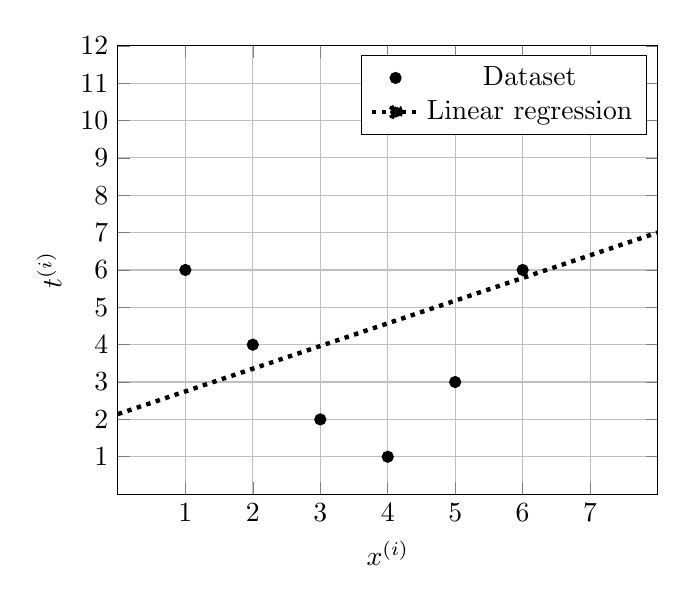
\begin{tikzpicture}
    \begin{axis}[
      xlabel={$x^{(i)}$},
      ylabel={$t^{(i)}$},
      xmin=0, xmax=8, 
      ymin=0, ymax=12,
      xtick={1,2,3,4,5,6,7},
      ytick={1,2,3,4,5,6,7,8,9,10,11,12},
      grid=both,
      mark=*,
      ]
      
      \addplot[only marks] table {
        1 6
        2 4
        3 2
        4 1
        5 3
        6 6
        7 10
      };
      \addlegendentry{Dataset}
	% question 1.5
      \addplot [dotted, domain=0:8, samples=2, ultra thick] {0.607142857*x + 2.142857143};
      \addlegendentry{Linear regression} //// mark=*????
    \end{axis}
  \end{tikzpicture}
  \caption{Scatter plot of $x^{(i)}$ vs. $t^{(i)}$}
\end{figure}
%%%%%%%%%%%%%%%%%%%%%%%%%%%%%%%%%%%%%%%%%%%%%%%%%%%%
%%%%%%%%%%%%%%%%%%%%%%%%%%%%%%%%%%%%%%%%%%%%%%%%%%%%
%%%%%%%%%%%%%%%%%%%%%%%%%%%%%%%%%%%%%%%%%%%%%%%%%%%%


\section{Least Squares}
\subsection{}
\begin{align*}
g_w(\vec{x}) &= \vec{x}\vec{w} \\
&= \begin{bmatrix} x^{(i)} & 1 \end{bmatrix} \begin{bmatrix} w \\ b \end{bmatrix} \\ %%% check the index xi ***
&= wx + (1)b \\
&= g_{w, b} (x) \\
\implies & \boxed{	 \vec{w} = 	 \begin{bmatrix} w \\ b \end{bmatrix}	} 
\end{align*}


\subsection{}

\begin{align*}
X\vec{w} - \vec{t} &=  \begin{bmatrix} x^{(1)} & 1 \\ x^{(2)} & 1 \\ \vdots & \vdots \\ x^{(N)} & 1 \end{bmatrix}  \begin{bmatrix} w \\ b \end{bmatrix} -  \begin{bmatrix} t^{(1)} \\ t^{(2)} \\ \vdots \\ t^{(N)} \end{bmatrix} \\
&= \sum_{i=1}^N  \begin{bmatrix} x^{(i)} & 1 \end{bmatrix} \vec{w} - t^{(i)} \\
&= \sum_{i=1}^N  x^{(i)} w + b - t^{(i)} \\
\implies || X\vec{w} - \vec{t} ||^2 &= \sum_{i=1}^N  (x^{(i)} w + b - t^{(i)})^2 \\
\nabla_{\vec{w}}  || X\vec{w} - \vec{t} ||^2 &= \begin{bmatrix} \frac{\partial || X\vec{w} - \vec{t} ||^2}{\partial w} \\ \\ \frac{\partial || X\vec{w} - \vec{t} ||^2}{\partial b} \end{bmatrix} \\
&= \begin{bmatrix} \sum_{i=1}^N  \frac{\partial }{\partial w} (x^{(i)} w + b - t^{(i)})^2 \\ \\  \sum_{i=1}^N  \frac{\partial }{\partial b} (x^{(i)} w + b - t^{(i)})^2 \end{bmatrix} \\
&= \begin{bmatrix} \sum_{i=1}^N  2(x^{(i)} w + b - t^{(i)}) \cdot (x^{(i)}) \\  \sum_{i=1}^N  2(x^{(i)} w + b - t^{(i)}) \end{bmatrix} \\
&= 2  \begin{bmatrix} x^{(i)} \\ 1 \end{bmatrix} ( X \vec{w} - \vec{t} ) \\
&= \boxed{ 2 X^T (X \vec{w} - \vec{t}	)}
\end{align*}




\subsection{}
Setting the derived loss function to zero,
$$0 = 2 X^T (X \vec{w} - \vec{t}) $$
{Thus $\vec{w^*}$ must satisfy: \\
$$ 0 = 2 X^T X \vec{w^*} - 2 X^T \vec{t}$$


\subsection{}
Assuming that $X^T X$ is invertible,
\begin{align*}
0 &= 2 X^T X \vec{w^*} - 2 X^T \vec{t} \\
2 X^T \vec{t} &= 2 X^T X \vec{w^*} \\
X^T \vec{t} &= X^T X \vec{w^*}  \\
 \vec{w^*} &= (X^T X)^{-1} X^T \vec{t} 
\end{align*}



\section{Regularized Linear Regression Model}

\subsection{}
\begin{align*}
A &= \sum_{i=1}^N \vec{x}^{(i)}   \vec{x}^{(i)^T} \\
&= \sum_{i=1}^N \begin{bmatrix} x_1^{(i)} \\ \vdots \\ x_d^{(i)} \end{bmatrix} \begin{bmatrix} x_1^{(i)} & \cdots & x_d^{(i)} \end{bmatrix} \\ &= \sum_{i=1}^N \begin{bmatrix}
x_1^{(i)} x_1^{(i)} & \cdots & x_1^{(i)} x_d^{(i)} \\
\vdots & \ddots & \vdots \\
x_d^{(i)} x_1^{(i)} & \cdots & x_d^{(i)} x_d^{(i)} 
\end{bmatrix} \\
&= \begin{bmatrix}
x_1^{(1)} x_1^{(1)} & \cdots & x_1^{(1)} x_d^{(1)} \\
\vdots & \ddots & \vdots \\
x_d^{(1)} x_1^{(1)} & \cdots & x_d^{(1)} x_d^{(1)} 
\end{bmatrix}
+
\begin{bmatrix}
x_1^{(2)} x_1^{(2)} & \cdots & x_1^{(2)} x_d^{(2)} \\
\vdots & \ddots & \vdots \\
x_d^{(2)} x_1^{(2)} & \cdots & x_d^{(2)} x_d^{(2)} 
\end{bmatrix}
+ \cdots +
\begin{bmatrix}
x_1^{(N)} x_1^{(N)} & \cdots & x_1^{(N)} x_d^{(N)} \\
\vdots & \ddots & \vdots \\
x_d^{(N)} x_1^{(N)} & \cdots & x_d^{(N)} x_d^{(N)} 
\end{bmatrix} \\
\implies A &=  \begin{bmatrix}
\sum_{i=1}^N x_1^{(i)} x_1^{(i)} & \cdots & \sum_{i=1}^N x_1^{(i)} x_d^{(i)} \\
\vdots & \ddots & \vdots \\
\sum_{i=1}^N x_d^{(i)} x_1^{(i)} & \cdots & \sum_{i=1}^N x_d^{(i)} x_d^{(i)} 
\end{bmatrix}
\end{align*}






\subsection{}
Given:
\begin{align*}
\mathcal{E}(\vec{w}, D) &= \frac{1}{2N} \sum_{i=1}^N (g_{\vec{w}} (\vec{x}^{(i)}) - t^{(i)} )^2 + \frac{\lambda}{2} || \vec{w} || _2^2 \\
g_{\vec{w}} &= \vec{x^{(i)^T}} \vec{w} \\
A &= \sum_{i=1}^N \vec{x}^{(i)}   \vec{x}^{(i)^T} \\
\vec{b} &= \sum_{i=1}^N t^{(i)} \vec{x}^{(i)} \text{,} \\
%%%
\nabla \mathcal{E}(\vec{w}, D) &= \nabla \left( \frac{1}{2N} \sum_{i=1}^N g_{\vec{w}} (\vec{x}^{(i)}) - t^{(i)} )^2 + \frac{\lambda}{2} || \vec{w} || _2^2 \right) \\
&= \nabla \left( \frac{1}{2N} \sum_{i=1}^N g_{\vec{w}} (\vec{x}^{(i)}) - t^{(i)} )^2 \right) + \nabla \left( \frac{\lambda}{2} || \vec{w} || _2^2 \right) \\
&=  \frac{1}{2N} \sum_{i=1}^N \nabla \left( (\vec{x^{(i)^T}} \vec{w} - t^{(i)} )^2 \right) + \frac{\lambda}{2} 2w \\
&=  \frac{1}{2N} \sum_{i=1}^N \nabla \left( ((\vec{x^{(i)^T}} \vec{w})^2 - 2 \vec{x^{(i)^T}} \vec{w} t^{(i)} + (t^{(i)})^2 )^2 \right) + \lambda w \\
&= \frac{1}{N} ( \sum_{i=1}^N \vec{x}^{(i)}   \vec{x}^{(i)^T} \vec{w} - \sum_{i=1}^N t^{(i)} \vec{x}^{(i)} ) + \lambda w \\
&= \frac{1}{N} (A \vec{w} - \vec{b}) + \lambda w
\end{align*}













\subsection{}
Setting $\nabla \mathcal{E} (\vec{w}, D)$ to zero and using $\vec{w}^*$ which minimizes the loss,
\begin{align*}
\nabla \mathcal{E} (\vec{w}, D) &=  \frac{1}{N} (A \vec{w}^* - \vec{b}) + \lambda \vec{w}^* = 0 \\
0 &= \frac{1}{N} A \vec{w}^* - \frac{1}{N} \vec{b} + \lambda \vec{w}^* \\
&= A \vec{w} - \vec{b} + \lambda N I \vec{w}^* \\
\implies \vec{b} &= (A + \lambda N I) \vec{w}^*
\end{align*}








\subsection{}
We will prove that all eigenvalues of A are non-negative. If A is positive semi-definite, then all its eigenvalues will be non-negative (ECE421 tutorial \#1 notes).

\begin{align*}
\vec{v}^T A \vec{v} \geq 0 & \forall \vec{v} \epsilon \mathbb{R}^n \implies A \; \text{is positive semi-definite.} \\
\text{Recall that:} \; A &=  \sum_{i=1}^N \vec{x}^{(i)}   \vec{x}^{(i)^T}. \\
\vec{v}^T A \vec{v} &= \vec{v}^T \left( \sum_{i=1}^N \vec{x}^{(i)} \vec{x}^{(i)^T} \right) \vec{v} \\
&= \sum_{i=1}^N (\vec{v}^T \vec{x}^{(i)} ) (\vec{x}^{(i)^T} \vec{v} ) \\
&= \sum_{i=1}^N (\vec{v}^T \vec{x}^{(i)} )^2 \geq 0 \qquad \implies \text{A's eigenvalues are non-negative}.
\end{align*}





\subsection{}
Let $ \textcolor{blue}{A} \vec{v}  = \textcolor{purple}{\alpha} \vec{v} $ where $ \alpha $ is a non-negative eigenvalue of A (as proved in \textbf{3.4}) and $\vec{v}$ be an eigenvector of A.


\begin{align*}
\textcolor{blue}{(A + \lambda N I_d)} \vec{v} &= A \vec{v} + \lambda N \vec{v} \\
&= \alpha \vec{v} + \lambda N \vec{v} \\
&= \textcolor{purple}{(\alpha + \lambda N)} \vec{v}
\end{align*}
$\alpha \geq 0 $ from \textbf{3.4} and $\lambda N > 0$. Thus, none of the eigenvalues $\textcolor{purple}{(\alpha + \lambda N)}$ of the matrix $\textcolor{blue}{(A + \lambda N I_d)}$ are zero, so the matrix $\textcolor{blue}{(A + \lambda N I_d)}$ is invertible.


\subsection{}
Using the result of \textbf{3.3},
\begin{align*}
(A + \lambda N I_d) \vec{w}^* &= \vec{b} \\
\implies \vec{w}^* &= (A + \lambda N I_d)^{-1} \vec{b}
\end{align*}





\end{document}